\documentclass{article}
\usepackage{tikz}
\usetikzlibrary{positioning}

\begin{document}

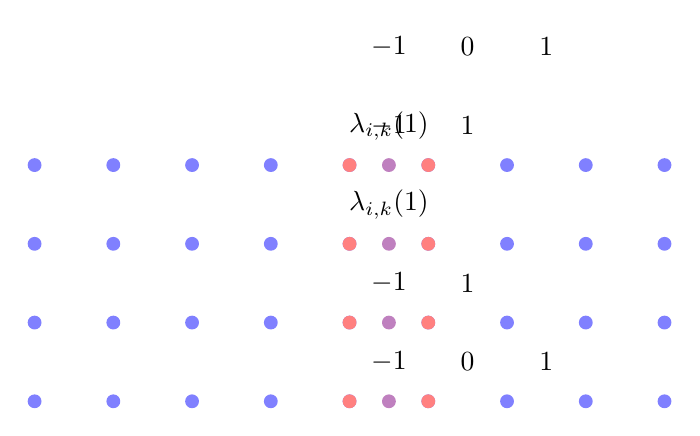
\begin{tikzpicture}[node distance=2cm]
    % Define styles for different types of nodes
    \tikzstyle{dot} = [circle, fill=blue!50, minimum size=5pt, inner sep=0pt]
    \tikzstyle{red_dot} = [circle, fill=red!50, minimum size=5pt, inner sep=0pt]
    \tikzstyle{purple_dot} = [circle, fill=violet!50, minimum size=5pt, inner sep=0pt]

    % Draw the horizontal line with dots
    \foreach \x in {-4,...,-1,0,1,...,4}
        \node[dot] (d\x) at (\x,0) {};
    
    % Draw the red dots
    \foreach \x in {0,1}
        \node[red_dot] (r\x) at (\x,0) {};
    
    % Draw the purple dot
    \node[purple_dot] (p) at (0.5,0) {};
    
    % Draw the labels
    \node at (0.5,0.5) {$-1$};
    \node at (1.5,0.5) {$0$};
    \node at (2.5,0.5) {$1$};
    
    % Draw the second row
    \foreach \x in {-4,...,-1,0,1,...,4}
        \node[dot] (d\x) at (\x,1) {};
    
    % Draw the red dots
    \foreach \x in {0,1}
        \node[red_dot] (r\x) at (\x,1) {};
    
    % Draw the purple dot
    \node[purple_dot] (p) at (0.5,1) {};
    
    % Draw the labels
    \node at (0.5,1.5) {$-1$};
    \node at (1.5,1.5) {$1$};
    
    % Draw the third row
    \foreach \x in {-4,...,-1,0,1,...,4}
        \node[dot] (d\x) at (\x,2) {};
    
    % Draw the red dots
    \foreach \x in {0,1}
        \node[red_dot] (r\x) at (\x,2) {};
    
    % Draw the purple dot
    \node[purple_dot] (p) at (0.5,2) {};
    
    % Draw the labels
    \node at (0.5,2.5) {$\lambda_{i,k}(1)$};
    \node at (0.5,3.5) {$-1$};
    \node at (1.5,3.5) {$1$};
    
    % Draw the fourth row
    \foreach \x in {-4,...,-1,0,1,...,4}
        \node[dot] (d\x) at (\x,3) {};
    
    % Draw the red dots
    \foreach \x in {0,1}
        \node[red_dot] (r\x) at (\x,3) {};
    
    % Draw the purple dot
    \node[purple_dot] (p) at (0.5,3) {};
    
    % Draw the labels
    \node at (0.5,3.5) {$\lambda_{i,k}(1)$};
    \node at (0.5,4.5) {$-1$};
    \node at (1.5,4.5) {$0$};
    \node at (2.5,4.5) {$1$};
\end{tikzpicture}

\end{document}